\documentclass[twocolumn,a4paper,dvipdfmx]{ieicejsp}
\usepackage{cite}
\usepackage{graphicx}
\usepackage{times}
\usepackage{url}
\usepackage[dvipdfmx]{hyperref}
\date{}
\title{}
\hypersetup{
 pdfauthor={shun},
 pdftitle={},
 pdfkeywords={},
 pdfsubject={},
 pdfcreator={Emacs 28.2 (Org mode 9.5.5)}, 
 pdflang={Ja}}
\begin{document}

\title{研究タイトル}
\author{山近 駿}
\affliate{所属大学・学部}
\maketitle


\section{Linkselfieについて}
\label{sec:orgaaf59af}
\subsection{P(Point:結論・要点)}
\label{sec:org469e492}
LinkSelfieの実験設定はアルゴリズムの効率性を示せていない

\subsection{R(Reason:理由)}
\label{sec:orge4837b6}
Linkselfie の提案する実験設定は、均等配分戦略(VanillaNB)のような単純
なベースライン手法と比較して、資源消費の削減や性能向上と
いう点で優位性を示せていないから。

Linkselfieは、そのベースラインである均等配分手法(VanillaNB)に、特に
理由なく過剰な試行回数 T=200(各リンクに2,000バウンス)を設定し、その
上でより少ない資源で同等以上の性能を目指すという形で優位性を示そうとし
ている。しかしT を大幅に削減した均等配分戦略(Vanilla 20NB、Vanilla
4NB つまり各リンクに200バウンス、40バウンス)をLinkselfieと同じ実験設
定下で実験すると結果が得られた。

\begin{itemize}
\item 最適リンクの判別率: Vanilla 4NB、Vanilla 20NBはLinkselfieと同程度の
最適リンク判別率を達成。

\item 量子資源消費: Vanilla 20NB、Vanilla 4NBは、Linkselfieと比較して
劇的に少ない総バウンス数(量子資源)でアルゴリズムが終了している。

\item 忠実度推定精度: Vanilla 20NBがLinkselfieと同等の高い忠実度推定精度
(相対誤差 1\% 未満)を実現できている。
\end{itemize}

つまり、Linkselfieが解決しようとした「最小限の量子資源で、最も高忠実度
なリンクを特定し、その忠実度を正確に推定する」という目的は、Linkselfie
よりもはるかに少ない資源と単純な戦略(Vanilla 20NB)によって、十分達成
可能である。

このことから、Linkselfieの実験設定ではLinkselfieのアルゴリズムが、資源
効率と性能の点で均等配分戦略を上回ることができていない、または均等配分
戦略が過剰な資源配分を要求しているという前提が崩れているため、
アルゴリズムの効率性を示せていない。
\subsection{E(Example:具体例)}
\label{sec:org33b985b}
最小限の量子資源で、最も高忠実度なリンクを特定し、その忠実度を正確に推
定するアルゴリズムを設計するというlinkselfieの目的が均等配分戦略で実現
できていることをシュミレーションによって示す。

VanillaNB は、各リンクを同じ回数だけベンチマークする単純な手法であり、
linkselfieではその繰り返し回数Tが200に設定されていた。

繰り返し回数の少ない均等配分戦略アルゴリズムの有効性を評価するために、
今回の実験ではT=4とT=20のVanilla 4NB、Vanilla 20NBを実装し、linkselfie
とこれらの均等配分戦略を比較する。

実験設定や各パラメータ設定はlinkselfieと同じ実験設定で行なった。

\begin{itemize}
\item 実験の設定
\end{itemize}
我々は 2 つのノード(ソース S とデスティネーション D)から成る単純なネッ
トワークを構築し、その間に L 本のエンタングルメントリンクを配置する。
各リンクは4種類の標準的な量子ノイズモデルに従う
Depolarizing Noise(脱分極ノイズ)
Dephasing Noise(位相緩和ノイズ)
Amplitude Damping Noise(振幅減衰ノイズ)
Bit-Flip Noise(ビット反転ノイズ)
これらのノイズモデルのパラメータは、同一の忠実度値に対応するように変換
されている。






\begin{figure}[h]
\centering
\begin{minipage}[b]{0.45\columnwidth}
\centering
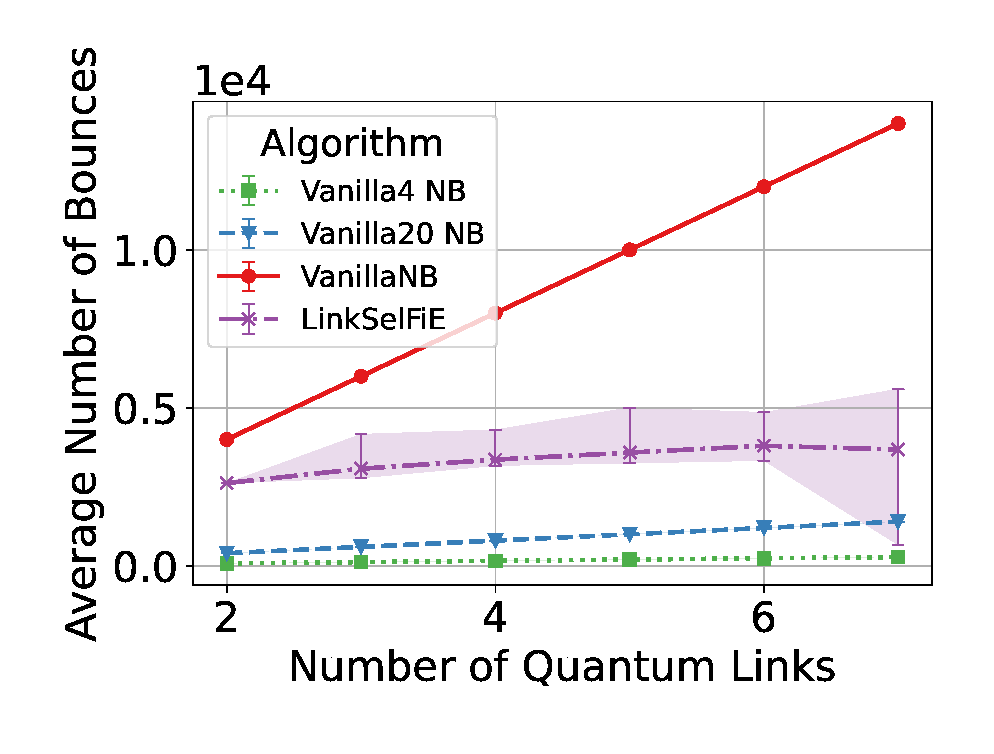
\includegraphics[width=\textwidth]{figure/plot_cost_vs_path_num_AmplitudeDamping.eps}
\caption{\tiny plot\_cost\_vs\_path\_num\_AmplitudeDamping.eps}
\end{minipage}
\hfill
\begin{minipage}[b]{0.45\columnwidth}
\centering
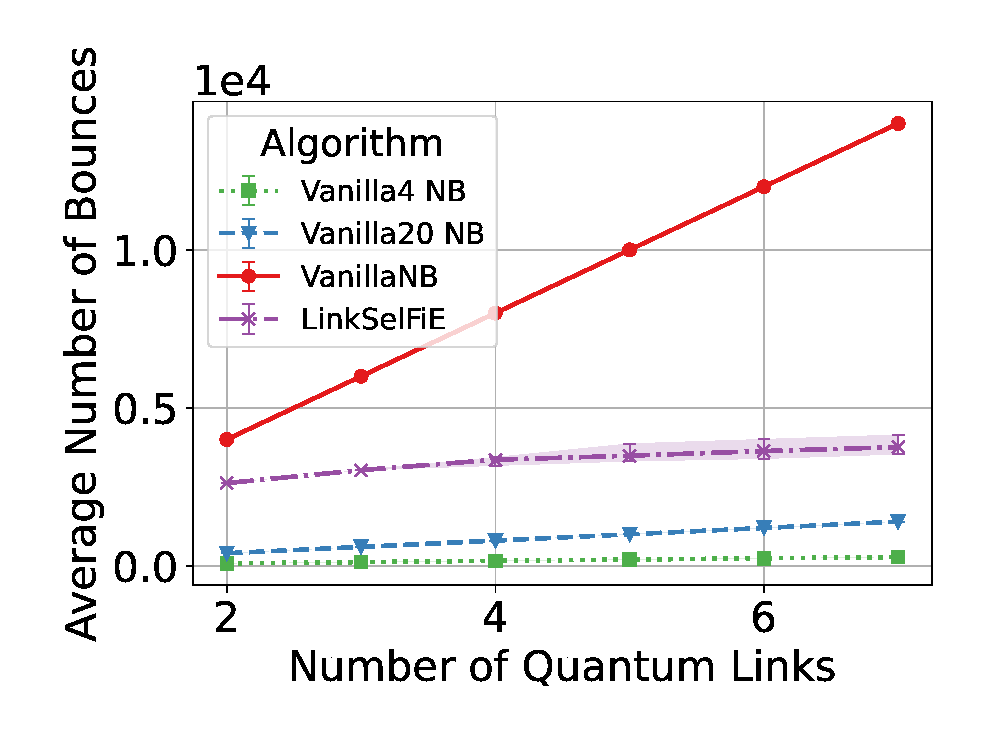
\includegraphics[width=\textwidth]{figure/plot_cost_vs_path_num_BitFlip.eps}
\caption{\tiny plot\_cost\_vs\_path\_num\_BitFlip.eps}
\end{minipage}
\end{figure}

\begin{figure}[h]
\centering
\begin{minipage}[b]{0.45\columnwidth}
\centering
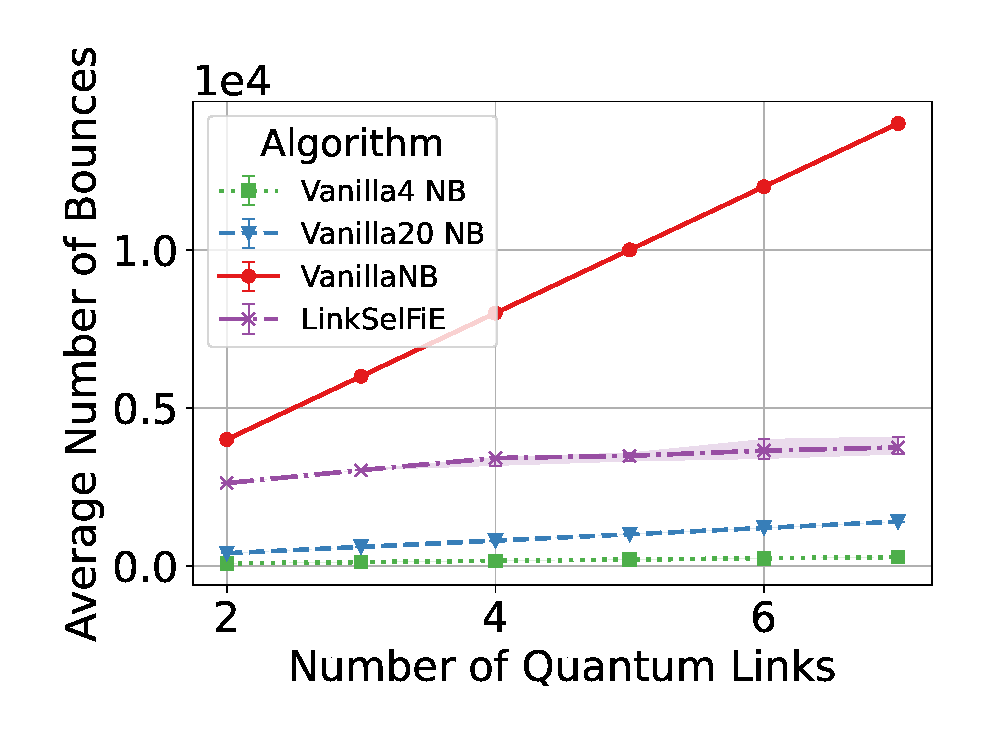
\includegraphics[width=\textwidth]{figure/plot_cost_vs_path_num_Dephase.eps}
\caption{\tiny plot\_cost\_vs\_path\_num\_Dephase.eps}
\end{minipage}
\hfill
\begin{minipage}[b]{0.45\columnwidth}
\centering
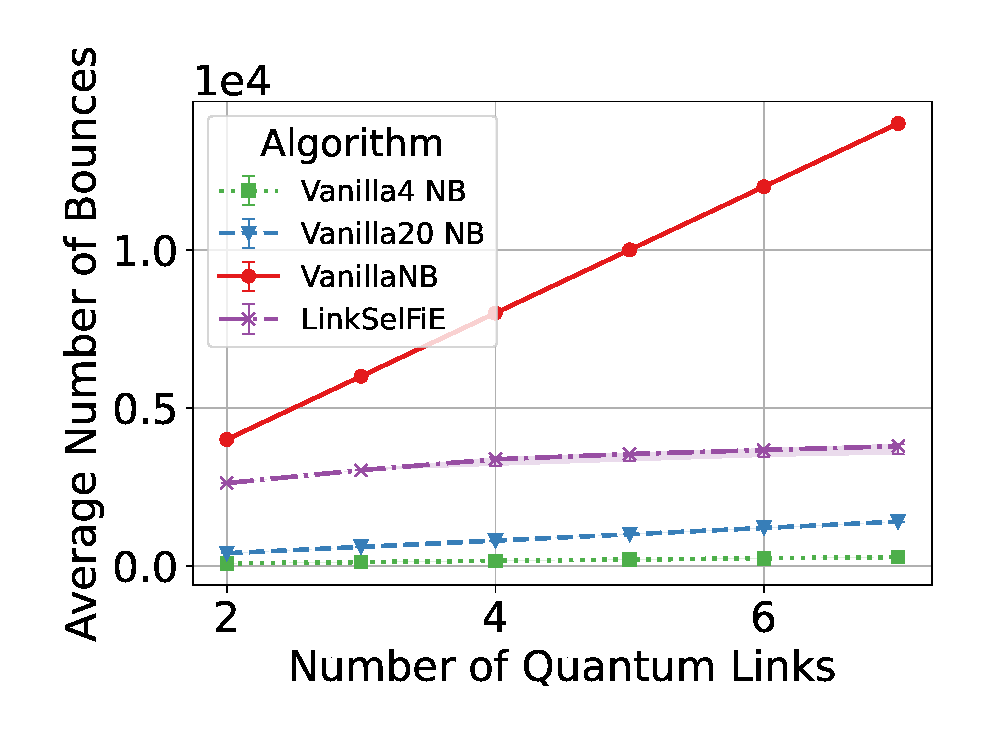
\includegraphics[width=\textwidth]{figure/plot_cost_vs_path_num_Depolar.eps}
\caption{\tiny plot\_cost\_vs\_path\_num\_Depolar.eps}
\end{minipage}
\end{figure}
図1,2,3,4 cost vs path\_num

まず、これらのリンク選択アルゴリズムにおける量子リソース消費を評価する。
忠実度ギャップ Δ = 0.05 を固定し、複数の量子エンタングルメントリンクで
接続された2ノードの量子ネットワークをシミュレートする。それぞれのリン
クは、忠実度 1, 1 − Δ, 1 − 2Δ, …, 1 − (L − 1)Δ を持つものとする。その
後、各リンク選択アルゴリズムをネットワークに適用し、さまざまな L の値
に対してアルゴリズムが終了する際の量子リソース消費量を測定する。ここで、
量子リソース消費量の指標として総バウンス数を使用し、結果は 10 回の試行
の平均をとった。Vanilla 4NB、Vanilla 20NBがlinkselfieよりも少ない資源
で配分できていることがわかる。バウンス数はL = 7のときにVanilla 20NB
でlinkselfieの半分以下、Vanilla 4NBは1/10ほどである。


\begin{figure}[h]
\centering
\begin{minipage}[b]{0.45\columnwidth}
\centering
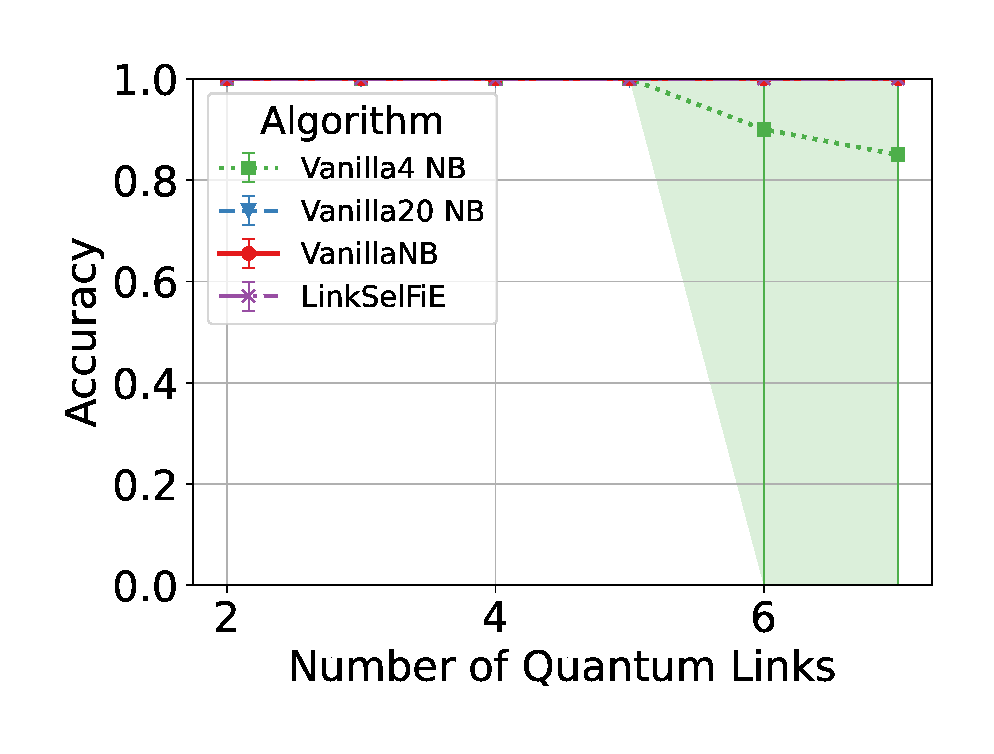
\includegraphics[width=\textwidth]{figure/plot_accuracy_vs_path_num_AmplitudeDamping.eps}
\caption{\tiny plot\_accuracy\_vs\_path\_num\_AmplitudeDamping.eps}
\end{minipage}
\hfill
\begin{minipage}[b]{0.45\columnwidth}
\centering
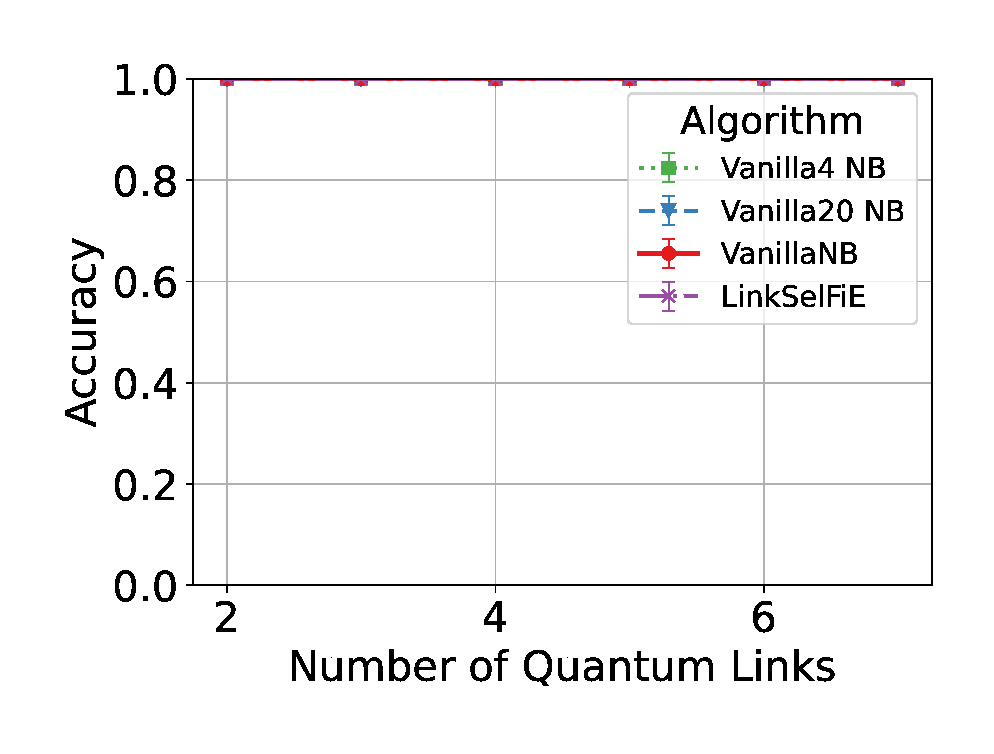
\includegraphics[width=\textwidth]{figure/plot_accuracy_vs_path_num_BitFlip.eps}
\caption{\tiny plot\_accuracy\_vs\_path\_num\_BitFlip.eps}
\end{minipage}
\end{figure}

\begin{figure}[h]
\centering
\begin{minipage}[b]{0.45\columnwidth}
\centering
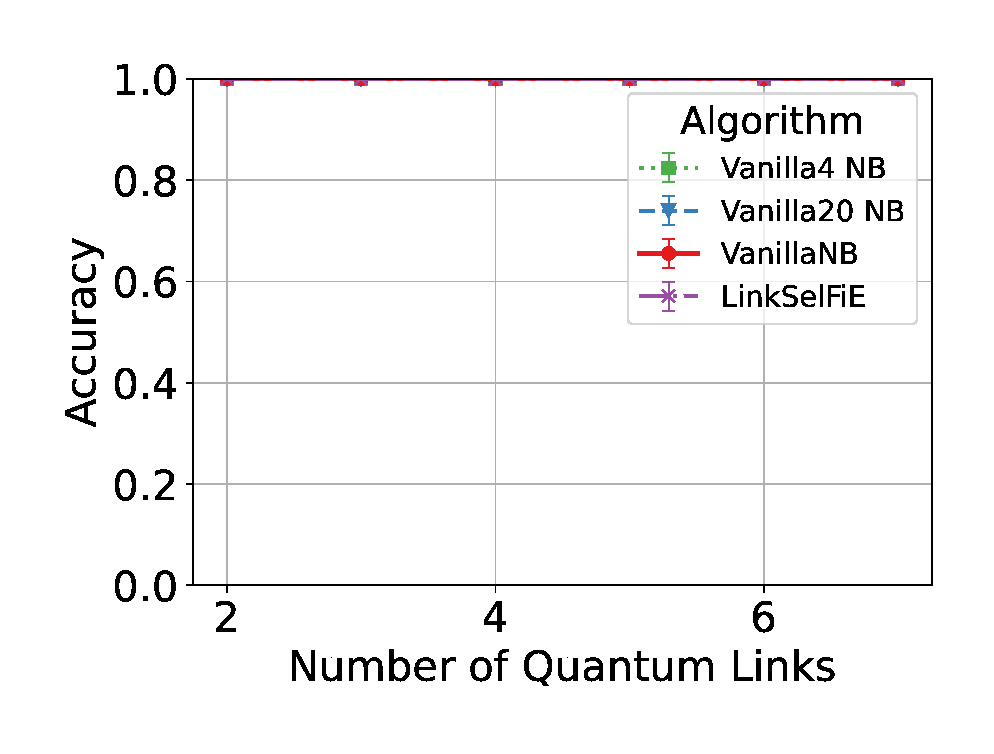
\includegraphics[width=\textwidth]{figure/plot_accuracy_vs_path_num_Dephase.eps}
\caption{\tiny plot\_accuracy\_vs\_path\_num\_Dephase.eps}
\end{minipage}
\hfill
\begin{minipage}[b]{0.45\columnwidth}
\centering
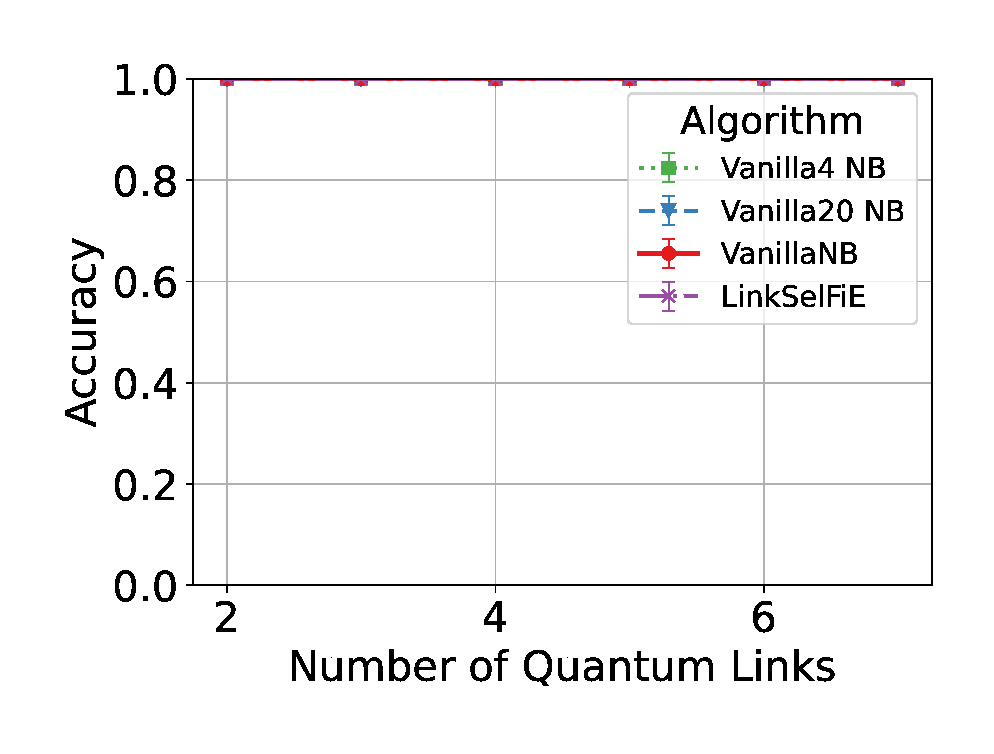
\includegraphics[width=\textwidth]{figure/plot_accuracy_vs_path_num_Depolar.eps}
\caption{\tiny plot\_accuracy\_vs\_path\_num\_Depolar.eps}
\end{minipage}
\end{figure}
図5,6,7,8 accuracy vs path\_num

次に、リンク選択アルゴリズムにおける最適リンク判別率を評価する。忠実度
ギャップ Δ = 0.05 を固定し、複数の量子エンタングルメントリンクで接続さ
れた2ノードの量子ネットワークをシミュレートする。それぞれのリンクは、
忠実度 1, 1 − Δ, 1 − 2Δ, …, 1 − (L − 1)Δ を持つものとする。その後、各
リンク選択アルゴリズムをネットワークに適用し、さまざまな L の値に対し
てアルゴリズムの最適リンク判別率を測定する。ここで最適リンク判別率とは
アルゴリズムが真の最良パスを正しく選択できた確率のことである。結果は
10 回の試行の平均をとった。Vanilla 4NB、Vanilla 20NBではlinkselfieと同
等の判別率があることがわかる。
\begin{figure}[h]
\centering
\begin{minipage}[b]{0.45\columnwidth}
\centering
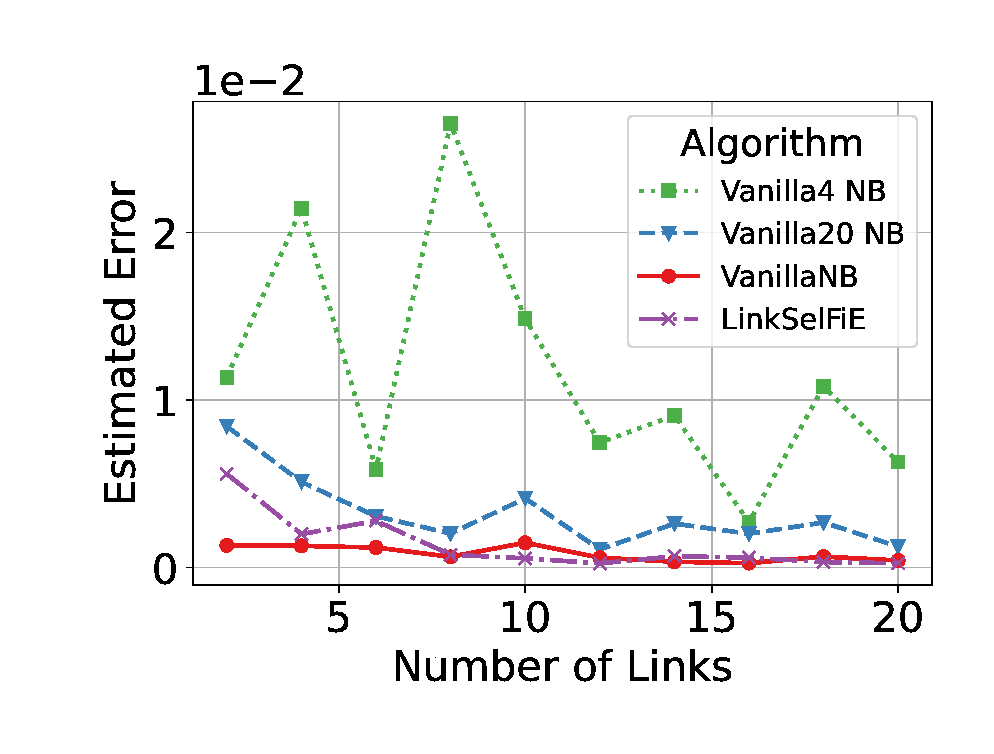
\includegraphics[width=\textwidth]{figure/plot_error_vs_path_num_AmplitudeDamping.eps}
\caption{\tiny plot\_accuracy\_vs\_path\_num\_AmplitudeDamping.eps}
\end{minipage}
\hfill
\begin{minipage}[b]{0.45\columnwidth}
\centering
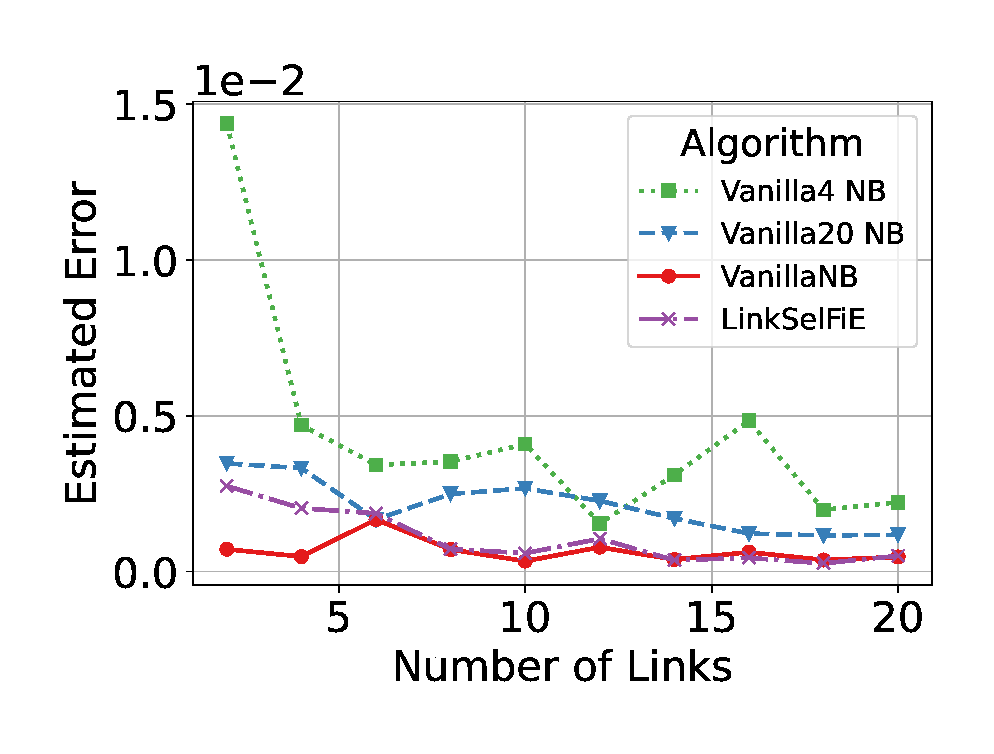
\includegraphics[width=\textwidth]{figure/plot_error_vs_path_num_BitFlip.eps}
\caption{\tiny plot\_accuracy\_vs\_path\_num\_BitFlip.eps}
\end{minipage}
\end{figure}

\begin{figure}[h]
\centering
\begin{minipage}[b]{0.45\columnwidth}
\centering
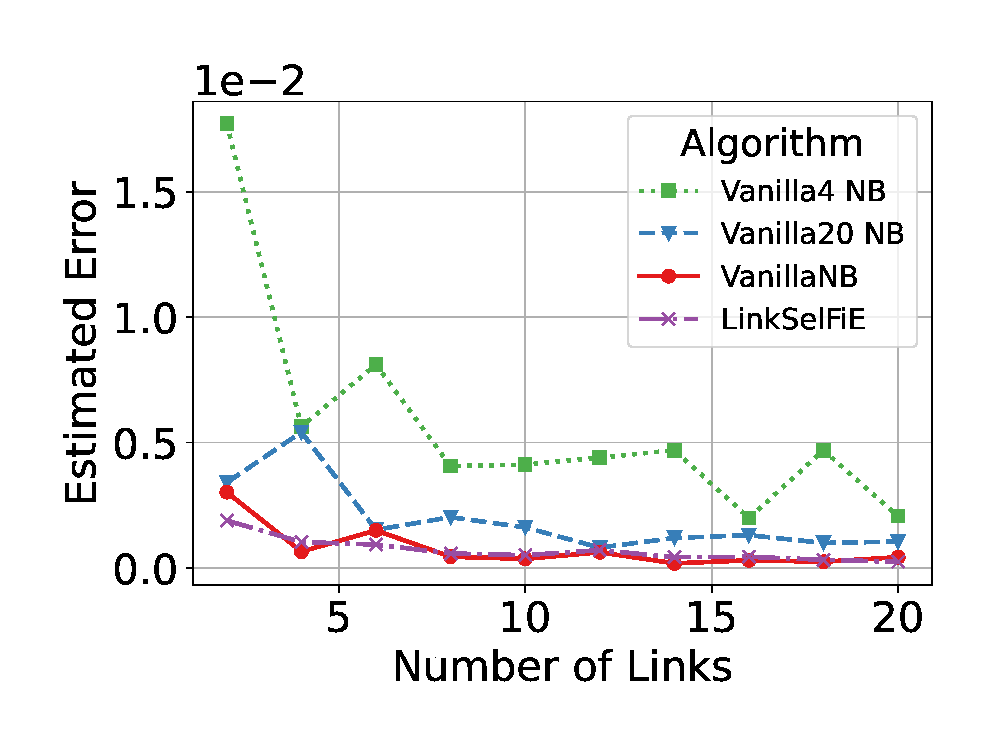
\includegraphics[width=\textwidth]{figure/plot_error_vs_path_num_Dephase.eps}
\caption{\tiny plot\_accuracy\_vs\_path\_num\_Dephase.eps}
\end{minipage}
\hfill
\begin{minipage}[b]{0.45\columnwidth}
\centering
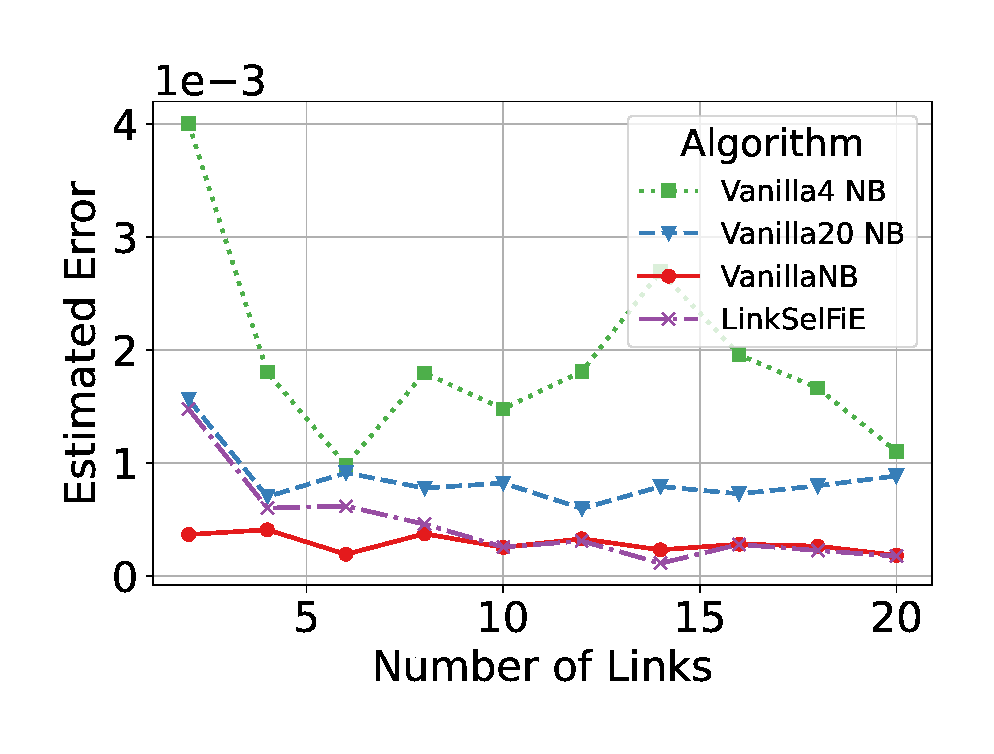
\includegraphics[width=\textwidth]{figure/plot_error_vs_path_num_Depolar.eps}
\caption{\tiny plot\_accuracy\_vs\_path\_num\_Depolar.eps}
\end{minipage}
\end{figure}
図9,10,11,12
Fidelity Estimation Accuracy
次に、各アルゴリズムの忠実度推定精度を評価する。
各リンクの平均忠実度はそれぞれ μ1 = 0.95 および μi = 0.85(i = 2, 3, …, L)と設定する。
各リンク i の忠実度 fᵢ は、平均 μᵢ、分散 1/4 のガウス分布からサンプリングされる。
その後、各アルゴリズムをこのネットワークに適用し、
各アルゴリズムが選択した最適リンクの推定忠実度を得る。
アルゴリズムが出力した推定忠実度を、真の忠実度と比較することで、
相対誤差(relative error)を求める。
リンク数 L を 2 から 20 まで変化させ、
各設定について 10 回の試行を行い、その平均値を結果として出力する。

linkselfieの論文では"LINKSELFIE の相対誤差は 1\% 未満であり、他のアルゴ
リズムと比較して有意な差は見られない。"と言及されていた。そうなのであ
れば、Vanilla 20NBの相対誤差も1\% 未満であり、linkselfieと比較して有意
な差は見られないと言える。




\subsection{P(Point:結論の繰り返し)}
\label{sec:orge37f4b6}
結果としてVanilla 20NBはlinkselfieよりもはるかに少ないリソースで最適リ
ンクを選択しつつ、同等レベルの忠実度推定精度を達成しており、リンク判別
だけならばVanilla 4NBでもある程度判別可能であるということが分かった。これ
は量子資源、最適リンクの特定、最適リンクの推定精度という観点で
linkselfieが均等配分手法を上回ることができていないことを示している。ゆ
えにLinkSelfieの実験設定は、アルゴリズムの効率性を示せていない


\subsection{補足}
\label{sec:org46703a0}
linkselfieの目的
\begin{itemize}
\item 最小限の量子資源で、最も高忠実度なリンクを特定し、その忠実度を正確に推定するアルゴリズムを設計する
\end{itemize}

"The main objective of this work is to efficiently estimate the fidelity of established entangled links."

"Our objective is to identify the link with the highest fidelity from a
link set and get its fidelity estimate while consuming as few quantum
resources as possible."



As expected, LINKSELFIE can not only identify the optimal link but
also evaluate its fidelity accurately. The relative error of
LINKSELFIE is less than 1\%, which has no significant difference
compared with other algorithms.

誤差(relative error)1\%未満で他の手法と同程度としており、linkselfie
レベルの誤差(0.003)の必要性は書かれていない。


\begin{itemize}
\item この文章が間違っている
\end{itemize}
Moreover, we perform extensive simulations under
various scenarios to corroborate that L INK S EL F I E outperforms
other existing methods in terms of both identifying the optimal
link and reducing quantum resource consumption.


\begin{itemize}
\item ネットワークベンチマーキング(NB)について
\end{itemize}
NBは、量子ネットワークのパフォーマンスを測定するための基礎的な手法であ
る。特に、ネットワークのリンク品質を評価するために、量子状態の「バウン
ス」実験を繰り返すプロトコルが利用される。ネットワークベンチマーキング
は、あるリンクを通してエンタングルメントを生成し、その状態を送信ノード
S から受信ノード D に何度も往復(bounce)させることにより、リンクの
「生存確率(survival probability)」を測定する。

実際、1 つのベンチマーク実験は、次のパラメータによって特徴づけられる:
\begin{itemize}
\item M:バウンス回数の集合(例:\{1, 2, 3, 4\})
\item T:各バウンス回数に対する繰り返し回数(repetition times)
\end{itemize}
ベンチマークの過程で、各 m∈M に対して T 回の測定を行い、対応する生存確
率 bm を記録する。
これらの観測値 \{b\_m\} は、理論的に次のような指数減衰モデルに従う:


\[
b_m = A p^{2m},
\]
ここで,

\begin{itemize}
\item \$A\$:測定および状態準備エラーの影響を表す定数,
\item \$p\$:量子チャネルの脱分極パラメータ(depolarizing parameter)
\end{itemize}


このとき,\(p\) の推定値 \(\hat{p}\) から,
リンクの平均忠実度(average fidelity)は次式で求められる:
\[
\hat{F} = \frac{1 + \hat{p}}{2}.
\]

linkselfieの論文でNBは量子ネットワーク内のリンク品質を評価するための基
本的手続きとして説明されており、全ての手法(VanillaNB, SuccElimNB,
LINKSELFIE)でこの NB をサブルーチンとして呼び出して動作する。

Network benchmarking (NB) is a fundamental procedure to evaluate the link quality in a quantum network.

\begin{itemize}
\item VanillaNB
\end{itemize}
VanillaNB benchmarks each link equally with the same number of repetitions (T = 200).
\begin{itemize}
\item Linkselfie
\end{itemize}
LINKSELFIE leverages network benchmarking (NB) as a subroutine to measure the fidelity of selected links.
\end{document}